\documentclass{mcmthesis}
\mcmsetup{CTeX = false,   % 使用 CTeX 套装时,设置为 true
        tcn = 88022, problem = B,
        sheet = true, titleinsheet = true, keywordsinsheet = false,
        titlepage = true, abstract = true}
\usepackage[english]{babel}
% \usepackage{fontspec}
\usepackage{palatino}
\usepackage{lipsum}
\title {How many languages}
\author{Zhao Yi, Peng Xutan, Chen Dengbo}
\date{\today}

\begin{document}
% \setmainfont{Times New Roman}
\begin{abstract}

  %\indent With the development of globalization, people get to know more about other tongues, so the research about the language rises. Recently, a multinational service company wants to expand to be more international and have employees who can speak different several languages. For this sake it needs to know the trends of global languages and wants to get advice about new offices's locations.\\
  \indent This paper establishes the XXX model to predict the trends of global languages and provide the best recommendations about the location of international office for a multinational company.\\
  \indent Firstly, in order to predict how languages of the world may vary over time, we build a force model and consider the influence a country gives to the other as a force, after getting the resultant force of this model, we can find how the ratio of languages of a country will change in the future. Using this model, we predict the trends of native speakers and total language speaks in the next 50 years and find that ... .\\
  \indent Secondly, based on the result our model produces, we use K-means algorithm to help us locate the best place for the company's global offices, using data collected from Twitter sampling. And we compare our recommendations with the global office choosen by world top 500 to verify our method and get great results.\\
  \indent Thirdly, we studied how would our model's results change with the type of our client company....
\begin{keywords}
  Force model, K-means clustering
\end{keywords}
\end{abstract}
\maketitle
\pagestyle{empty}
\newpage
\tableofcontents
\newpage
\pagestyle{fancy}
\setcounter{page}{1}
\section{Introduction}
\subsection{Background}
  \indent \indent Half of the world's population speak one of ten languages as their native language, although there are nearly 7,000 languages spoken on the earth. But with the influence of government, culture, economy and the impact of globalization, popularity of languages may change over the time. \\
  \indent A COO of a multinational service company wants to know the trends of global languages and locations for this company's new international offices. So we designed a multiple regression model and applied a fuzzy algorithm to help this company make the choice.
\subsection{Restatement of the Problem}
  \indent \indent We are required to build a model to predict the trends of global languages, including the number of speakers and the geographic distribution change of the top-10 languages. Then we need to decide where the new international offices of the company should be located, or take efforts to reduce the number of offices.

% \emph{center of percussion} [Brody 1986], \lipsum[5]

% \begin{Theorem} \label{thm:latex}
% \LaTeX
% \end{Theorem}
% \begin{Lemma} \label{thm:tex}
% \TeX .
% \end{Lemma}
% \begin{proof}
% The proof of theorem.
% \end{proof}

\section{Basic Assumptions}
\subsection{Assumption 1.}

  \indent \indent We assume that the land area of every country doesn't change during the period of time we study.

\subsection{Assumption 2.}

  \indent \indent We ignore unpredictable or low-probablity events that may cause great impact to languages trends.
 
% \begin{figure}[h]
% \small
% \centering
% 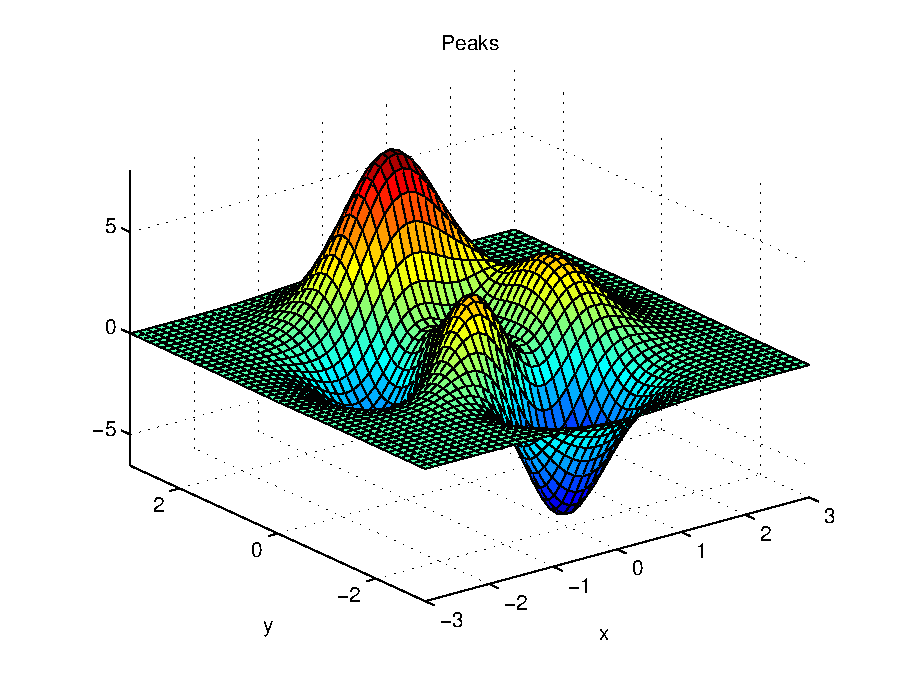
\includegraphics[width=12cm]{mcmthesis-aaa.eps}
% \caption{aa} \label{fig:aa}
% \end{figure}

% \lipsum[8] %\eqref{aa}
% \begin{equation}
% a^2 \label{aa}
% \end{equation}

% \begin{equation}
% e^{i \theta} = \cos \theta + i \sin \theta \label{bb}
% \end{equation}

% \[
%   \begin{pmatrix}{*{20}c}
%   {a_{11} } & {a_{12} } & {a_{13} }  \\
%   {a_{21} } & {a_{22} } & {a_{23} }  \\
%   {a_{31} } & {a_{32} } & {a_{33} }  \\
%   \end{pmatrix}
%   = \frac{{Opposite}}{{Hypotenuse}}\cos ^{ - 1} \theta \arcsin \theta \eqno(3)
% \]

% \lipsum[9]

% \[
%   p_{j}=\begin{cases} 
%   0,&\text{if $j$ is odd}\\
%   r!\,(-1)^{j/2},&\text{if $j$ is even}
%   \end{cases}
% \]

% \lipsum[10]

% \[
%   \arcsin \theta  =
%   \mathop{{\int\!\!\!\!\!\int\!\!\!\!\!\int}\mkern-31.2mu
%   \bigodot}\limits_\varphi
%   {\mathop {\lim }\limits_{x \to \infty } \frac{{n!}}{{r!\left( {n - r}
%   \right)!}}} \eqno (1)
% \]

\section{Analysis of the Problem}
  \indent \indent We consider the distribution of languages as the output of a function related to multiple factors, such as GDP, immigrants, population, imports, exports, and etc. These factors not only affect a country's language distribution, but also have an effect on other countries' languages. \\
  \indent So we build the model like this, assume ...

\section{Models and Methodology}
  \subsection{Time Series Prediction}
  \indent \indent In order to how the factors we mentioned above will change in the next 50 years, we use the well-known ARIMA model to predict them. ARIMA model, i.e autoregressive integrated moving average model, is a widely used method for predicting time series. Considering these factors change over the time, and to simplify this problem, we regard them as factors only related to time. The ARIMA model can be represented as following form.

  \begin{equation}
    \left(1-\sum^p_{i=1}\sigma_i L^i\right)(1-L)^d X_t = \left(1+\sum^q_{i=1}\theta_i L^i\right)\epsilon_t
  \end{equation}

  \indent In the equation above, $L$ stands for Lag Operator, d$\in$Z, d$>$0.

  \indent Considering these factors we use vary randomly and are related to many other factors, so they are not stationary variables and can not be directly used int ARIMA model. So we calculate the difference of factors we study and apply ARIMA model on them. After getting the forecast result we calculate the accumulation to restore prediction result. Take the GDP prediction for an example, we collect the GDP of countries from 2002 to 2016, calculate the difference of adjacent years and use the $auto.arima$ model of R language. After this ARIMA model gives us the prediction of how the difference of a country's GDP will change in the next 50 years, we calculate the accumulation of this prediction values and regard the final result as our prediction on this country's GDP.

\section{The Model Results}

\section{Validating the Model}

\section{Conclusions}

\section{A Summary}

\section{Evaluate of the Mode}

\section{Strengths and weaknesses}

\subsection{Strengths}
\begin{itemize}
\item \textbf{Applies widely}\\
This  system can be used for many types of airplanes, and it also
solves the interference during  the procedure of the boarding
airplane,as described above we can get to the  optimization
boarding time.We also know that all the service is automate.
\item \textbf{Improve the quality of the airport service}\\
Balancing the cost of the cost and the benefit, it will bring in
more convenient  for airport and passengers.It also saves many
human resources for the airline. \item \textbf{}
\end{itemize}
\subsection{Weaknesses}
\begin{itemize}
  \item \textbf{...}
  \item \textbf{...}
\end{itemize}


\begin{thebibliography}{99}
\bibitem{1} D.~E. KNUTH   The \TeX{}book  the American
Mathematical Society and Addison-Wesley
Publishing Company , 1984-1986.
\bibitem{2}Lamport, Leslie,  \LaTeX{}: `` A Document Preparation System '',
Addison-Wesley Publishing Company, 1986.
% \bibitem{3}\url{http://www.latexstudio.net/}
% \bibitem{4}\url{http://www.chinatex.org/}
\end{thebibliography}

\begin{appendices}

\section{First appendix}

\indent \indent Here are simulation programmes we used in our model as follow.\\

% \textbf{\textcolor[rgb]{0.98,0.00,0.00}{Input matlab source:}}
% \lstinputlisting[language=Matlab]{./code/mcmthesis-matlab1.m}

\section{Second appendix}

% some more text \textcolor[rgb]{0.98,0.00,0.00}{\textbf{Input C++ source:}}
% \lstinputlisting[language=C++]{./code/mcmthesis-sudoku.cpp}

\end{appendices}
\end{document}